\documentclass[letterpaper]{article}
\title{Auto Scaling Online Learning}
\date{}
\usepackage{balance}  % to better equalize the last page
\usepackage{graphicx}
\usepackage{times}    % comment if you want LaTeX's default font
\usepackage{url}      % llt: nicely formatted URLs
\usepackage{graphicx}
\usepackage{tabularx}
\usepackage{float}
\usepackage{color}
\usepackage{url}
\usepackage[noend]{algpseudocode}
\usepackage{algorithm}
\usepackage{verbatim}
\usepackage{mathtools}
\usepackage{caption}
\usepackage{subcaption}
%\usepackage{amsmath}
\let\proof\relax
\let\endproof\relax
\usepackage{amsthm}
\usepackage{thmtools}
\usepackage{xspace}
\usepackage{multirow}
\newcommand{\field}[1]{\mathbb{#1}} 
\newcommand{\hide}[1]{#1}
\newcommand{\pd}[2]{\frac{\partial #1}{\partial #2}}
\providecommand{\m}[1]{\mathbf{#1}}
\providecommand{\norm}[1]{\left\|#1\right\|}
\providecommand{\sign}[1]{\text{sign}\left(#1\right)}
\DeclareMathOperator*{\argmin}{arg\,min}
\providecommand{\what}{\m{\hat{w}}}

\begin{document}
\author{CSE 550 Project Proposal \\\\ Marco Tulio Correia Ribeiro, Shrainik Jain\\ 1323300, 1323338}
\maketitle

\section{Background and Prior work}
Online machine learning algorithms operate on a single instance at a time. They
have become particularly popular in natural language processing and applications
with streaming data, including classification, ranking, etc
\cite{Bordes:2005:HSE:2130928.2130979,
Carvalho:2006:SOL:1150402.1150466, Dredze:2008:CLC:1390156.1390190}. Online
learning is particularly interesting in the scenarios where data keeps streaming
in, such as a web search engine doing advertisement placement. It is also
interesting for scenarios where the whole dataset is too large to fit in main
memory, as online learning only operates on a single example at a time.

A lot of tasks that use online learning have a particular structure that can be 
broken down into 2 major components: 1 - Learning a model from data, and 2 -
making predictions according to the model. Going back to the web search engine
scenario as an example: the system needs to make predictions for every user
doing a query - and must also learn from the feedback given by those users.

This structure comes with multiple challenges. First, the 
the amount of data is always growing, so archiving it comes at a cost, both
because of storage constraints and computation constraints. A solution to this
is to just keep the current model in memory, and archive the rest in the
background. A second challenge is the
variable speed at which data streams in. Imagine a learning problem where in the
learning dataset is a live twitter stream for a hashtag. In this scenario the
rate at which the data comes in is a function of the popularity of the hashtag.
Finally, different applications have different costs for learning, and different
requirements for the latency of predictions.

\section{Proposed work}
The problem we will tackle in this project is the problem of automatically
handling the resources needed for online learning. The ideal system would
allocate the resources necessary to keep the prediction latency acceptable,
while at the same time learning appropriately. Finally, the system would be able
to handle bursts (such as increase in demand) and different learning
requirements for different systems.

Most of the current auto-scaling solutions handle services that are
easily replicated. Some examples include Amazon Web
Services\footnote{http://aws.amazon.com/}, which has an
option for auto-scaling, but that entails just spawning a new server with the
same app or the Google AppEngine, which scales appropriately depending on the
number of user requests. The assumption of easy replication is not true for
machine learning scenarios. Learning in a distributed scenario is a problem on
its own \cite{pserver1, pserver2}. Also, the system is two-tiered: there may be
a case where more learners are needed, and there may be a case where more
predictors are needed.

Our goal is to implement intelligent auto scaling while maintaining some
prediction service SOA, and some measurement of learning, with the minimum cost
possible. We plan on implementing a smart load-balancer that also handles the
spawning of new nodes, but we also don't want this load-balancer to be a
bottleneck, or a liability. Our current plan is to make it be a set of nodes.
We won't focus on the machine learning side of it, so we plan on using an
out-of-the-box fast machine learning solver: Vowpal Wabbit
\footnote{http://hunch.net/~vw/}. The challenges we see at the moment are:
\begin{itemize}
\item Determining when to start or shutdown more machines.
\item Determining the role the new machines should play, and making sure that
new predictors have a current model that is not too stale.
\item Ensuring that the system is fault taulerant.
\end{itemize}

\section{Roadmap}
Project Milestone: 
\begin{itemize} 
\item This is a fairly new problem and we would devote some initial time towards looking at existing similar solutions and formalizing the problem we are trying to solve.
\item Propose an initial design for the auto scaling service.
\end{itemize}
Short Presentation:
\begin{itemize} 
\item Setting up (possibly simulated) environment and
implement a first version of  our auto scaling system. 
\end{itemize}
Final Report:
\begin{itemize}
\item Detailed design specifications. 
\item Learning and results from the implementation (possibly simulated)
\end{itemize}

\bibliographystyle{plain}
\bibliography{references}
%\begin{figure}[h!]
%\centering
%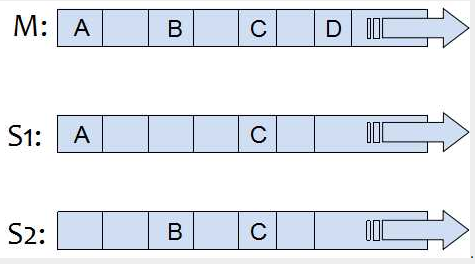
\includegraphics[scale=.5]{multipaxos.png}
%\caption{Illustration of multi-instance leader paxos. Source: StackOverflow.}
%\end{figure}

\end{document}
